\section{Codificador (Gray para Binário 3 bits)}
\subsection{Código de Gray}
A partir do que foi fornecido, foi possível realizar a construção da tabela verdade, que é mostrado a seguir:

\begin{table}[!htb]
    \centering
    \begin{tabular}{|c|c|c|c|c|c|}
        \hline
        \textbf{Gray} & \textbf{B2} & \textbf{B1} & \textbf{B0} \\
        \hline
        000           & 0           & 0           & 0           \\
        001           & 0           & 0           & 1           \\
        011           & 0           & 1           & 0           \\
        010           & 0           & 1           & 1           \\
        110           & 1           & 0           & 0           \\
        111           & 1           & 0           & 1           \\
        101           & 1           & 1           & 0           \\
        100           & 1           & 1           & 1           \\
        \hline
    \end{tabular}
    \caption{Tabela verdade do conversor de código de Gray para binário.}
    \label{table:GrayTable}
\end{table}

A partir da tabela verdade, conseguimos ver que o bit mais significativo (B2) é igual ao bit mais significativo do código de Gray (G2). Além disso, foi realizado o mapa de Karnaugh para os bits B1 e B0, que são mostrados a seguir:

\begin{figure}[!ht]
\centering

\begin{karnaugh-map}[4][2][1][$G_2$][$G_1$][$G_0$]
\minterms{1, 2, 5, 6}
\implicant{1}{5}
\implicant{2}{6}

\end{karnaugh-map}

\caption{Mapa de Karnaugh para o Bit $B_1$ do binário puro}
\end{figure}

\begin{figure}[!ht]
\centering

\begin{karnaugh-map}[4][2][1][$G_2$][$G_1$][$G_0$]
\minterms{1, 2, 4, 7}
\end{karnaugh-map}

\caption{Mapa de Karnaugh para o Bit $B_0$ do binário puro}
\end{figure}

Dessa forma, percebe-se que o bit $B_1$ e o bit $B_0$ podem ser expressos como:

\begin{equation}
    B_1 = \overline{G_2}G_1 + G_2\overline{G_1} = G_1 \oplus G_2
\end{equation}

\begin{equation}
    B_0 = \bar{G_2}\bar{G_1}G_0 + \bar{G_2}G_1\bar{G_0} + G_2\bar{G_1}\bar{G_0} + G_2G_1G_0 = G_0 \oplus G_1 \oplus G_2
\end{equation}

Para o esquemático, foi utilizado o software Quartus, resultando no esquemático mostrado na Figura \ref{fig:CodGray}.

\begin{figure}[!ht]
    \centering
    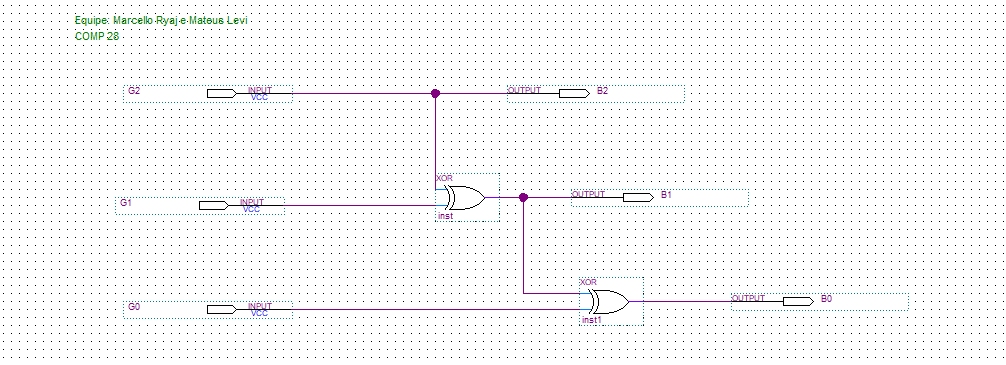
\includegraphics[width=0.8\textwidth]{fig/EsquematicoExercicio2.png}
    \caption{Esquemático do circuito para o Códificador Gray}
    \label{fig:CodGray}
\end{figure}

Após a realização do esquemático, foi possível realizar a simulação funcional, que é mostrada na Figura \ref{fig:SimulacaoExercicio2}.

\begin{figure}[!ht]
    \centering
    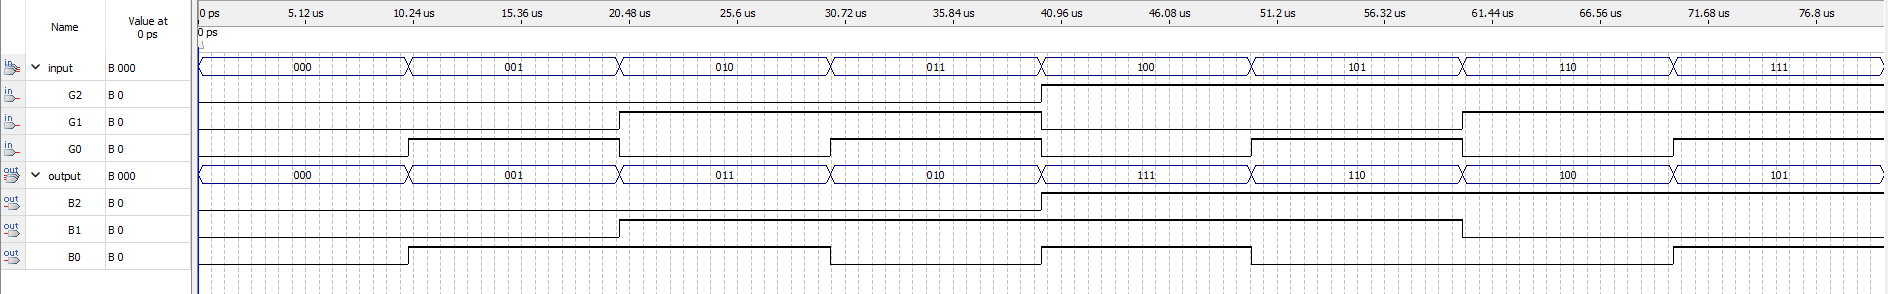
\includegraphics[width=1\textwidth]{fig/SimuExercicio2.png}
    \caption{Simulação funcional do circuito para o Códificador Gray}
    \label{fig:SimulacaoExercicio2}
\end{figure}

Comparando a simulação gerada com a tabela verdade produzida, é possível perceber que o circuito está funcionando corretamente, pois os bits de saída estão de acordo com o esperado para cada combinação de bits de entrada.




